\chapter{Modelling a single cardiac cell}

\def\ti{{\text{ti}}}
\def\Li{{\ce{Li^+}}}

\section{Overview of computational cellular modeling}
\label{sec:overv-comp-cell}


Modeling is a powerful tool to provide a quantitative insights to physiological
phenomena~\citep{fall2002,keener2008, winslow2011}.  The foundation to this
field is the Hodgkin-Huxley model (Sect.\ref{sec:Hodgkin-Huxley-1952-model})
developed for squid giant axon which has only 3 voltage-dependent
ionic components (\ce{Na+}, \ce{K+}, and \ce{Cl-}).


However, with more experimental data become available, more ionic components
have been revised and added.
Noblet (1962) introduced a HH-based model, with two different $\K$ currents of
opposite direction ~\citep{noble1962mhh}. This model, though simple and didn't
consider $\Ca$ current, can replicated the long AP in Purkinje fibers
(Sect.~\ref{sec:noble-model}).  Later on, in 1975, McAllister-Noble-Tsien
proposed an improved model with 9 ionic currents
(Sect.~\ref{sec:macall-noble-tsien}) target to Purkinje fibre
\citep{mcallister1975rea}.

Two years later, 1977, Beeler-Reuter (Sect.~\ref{sec:beeler-reuter-model})
proposed the first ventricular model with 4 ionic currents in which the second
inward current - mainly calcium current - was examined and play an important
role to the plateau shape of the cardiac AP. There is another important role
that make calcium being considered as the second-messenger agent is its role in
regulating the contractility of cardiac cells.

In 1985,~\citep{difrancesco1985mcea} proposed a landmark model of
Purkinje fibre, incorporating not only all ion channels, but also
ionic pumps and exchangers for the first time
(Sect.~\ref{sec:difr-noble-purk}). This is the base for the creation
of different models for SA node~\citep{noble1984msa}
(Sect.~\ref{sec:SA_node_Noble1984}) and atrial
cell~\citep{hilgemann1987,earm1990msa}
(Sect.\ref{sec:hilg-noble-model},\ref{sec:earm-noble-model}).

With the availability of voltage-clamp recordings from isolated myocytes,
extracellular ion concentrations can be controlled. This allows collecting a
plethora of data that show dynamics of ionic channels at different clamped
voltage and ion concentrations, leading to the first widely used model for
ventricular myocyte~\citep{luo1991mcap,luo1994dmc_a,luo1994dmc_b}
(Sect.~\ref{sec:luo-rudy-phase-1}, Sect.~\ref{sec:luo-rudy-phase-2}). Luo-Rudy
phase I model has 6 different ionic currents: $I_\na$ fast-inward Na current,
$I_\si$ slow-inward current, $I_\k$ a time-dependent delayed rectifier K
current, $I_{K1}$ time-independent inward rectifier current, $I_\Kp$ the plateau
K current, $I_\Kb$ the background K current. Luo-Rudy phase II model started
incorporating Na/Ca-exchanger, Na/K-ATPase pump, and SERCA-ATPase pump, $\Ca$
buffers, CICR and some modifications in ionic current components based on new
experimental data.

\begin{framed}
{\bf Ion channel model}:

For many years, Hodgkin-Huxley based-formula is the {\it de facto} for
deriving $V_m$-dependent kinetics of ion channels. However, its
limitation resides in the assumption that individual ion channels gate
independently, and two states only. This assumption can be relaxed by
using continuous-time Markov chain models, which comprise a number of
distinct states, loosely corresponding different major conformations
of the proteins. The transition rates between Markov states reflect
the free energy profile between two protein conformations, and must be
determined experimentally
({\it using voltage-clamp protocols, recording current responses, and
  adjusting transition rates using minimization algorithms to fit the
  data; single-channel patch-clamp data can be used to constraint
  Markov models})
(Sect. \ref{sec:i_na-channels}, Sect.~\ref{sec:IKr_current} and
Chap.~\ref{chap:dhpr-models}, Chap.~\ref{chap:ip3r-models}, and
Chap.~\ref{chap:ryr-models}).

Even though Markov models give better results, the aggregate number of
state equations may become large which consequently impose higher
computational load. An advanced method is described in
Sect.~\ref{sec:ultra-fast-markov}. 
\end{framed}

So far, Na/K-ATPase pump, Na/Ca-exchanger and SR Ca-ATPase pumps are
modeled as algebraic function of the relevant intracellular and
extracellular concentrations of $\Na, \Ca$ and $\K$ using
phenomenological Michaelis-Menten approach
(Sect.~\ref{sec:mich-ment-appr}). 

In 1998,~\citep{shannon1998} proposed a new model of SR Ca-ATPase pump
that included forward and reverse mode, each with its own
$\Ca$-binding constants and peak forward and reverse rate
(Sect.~\ref{sec:shannon-et-al}). Using Markovian approach, others
models for the pumps have also been approached: Na/K-ATPase
pump~\citep{smith2004}, SERCA pump~\citep{tran2009},
Na/Ca-exchanger~\citep{kang2004} (for more detail, read
Chap.~\ref{chap:models-pumps}, and Chap.~\ref{chap:serca-pumps-models}).
\textcolor{red}{Efforts to incorporate these models into whole-cell
  models are of particular important}.

So study the heart at some pathological condition, pH has been incorporated as a
new variable. The first was the phenomenological model in guinea pig
by~\citep{leem1999}. Models for Na/H ion exchanger, $\ce{Na-HCO3}$
cotransporter, Cl/OH exchanger, and anion exchanger have also been developed
by~\citep{crampin2006,crampin2006am}.
\textcolor{red}{Incorporating these study in whole-cell model would be
  great to study the effects, say acidosis in ischemia, on EC coupling and heart
  failure}.

The idea that SR $\Ca$ release sense a much higher calcium level than that in
the bulk has been incorporated into whole-cell model by ~\citep{jafri1998cad}.
It is the first model to incorporate mechanistic Markov models for both LCC and
RyRs, and to implement a ``restricted space'', a lumped compartment representing
all dyads into which $\Ca$ fluxes through RyRs and LCCs are directed before
diffusing into the myoplasm (Sect.~\ref{sec:jafri-rice-winslow}).

\begin{framed}
  {\bf high gain and graded $\Ca$ release}

  In {\bf local control theory}~\citep{wier1999}, the $\Ca$ elevation due to
  calcium influx is not global, but local at microdomain
  areas~\citep{lederer1990, stern1992tec, cheng1993cse}.
  \citep{lederer1990} first dubbed this microdomain as ``fuzzy space''. Later,
  it was coined the term {\it dyadic subspace} (or calcium release units/sites,
  CaRUs) at which a small number LCC in closed proximal to a cluster of RyRs. 
  The calcium influx triggers the opening of these $\Ca$-gated ion channels
  which then release a much higher calcium. This can show a {\bf high gain}
  (i.e. small influx trigger much higher release),
  Fig.\ref{fig:calcium_transient}, and {\bf gradeness} (i.e.
  the global elevation is the result of the recruitment of local elevations). 
  Fig.\ref{fig:calcium_transient} shown that sarcolemmal $\Ca$ influx appear to
  provide only 2.2\% of the total calcium elevation. The total SR calcium fluxes
  is $\sim 40$ times that of LCC current and other membrane fluxes
  \citep{cannell1994snu}.

  We use the term dyadic subspace because in this subspace, there are
  two fluxes: transarcolemmal influx of $\Ca$ and $\Ca$
  release from SR. Endoplasmic/Sarcoplasmic reticulum (ER/SR) is the major
  intracellular reservoir for $\Ca$. SR have many calcium release sites called
  RyR (ryadonine receptor) and IP3-gated $\Ca$-channels (inositol
  1,4,5-triphosphate). 
\end{framed}


\begin{figure}[hbt]
  \centerline{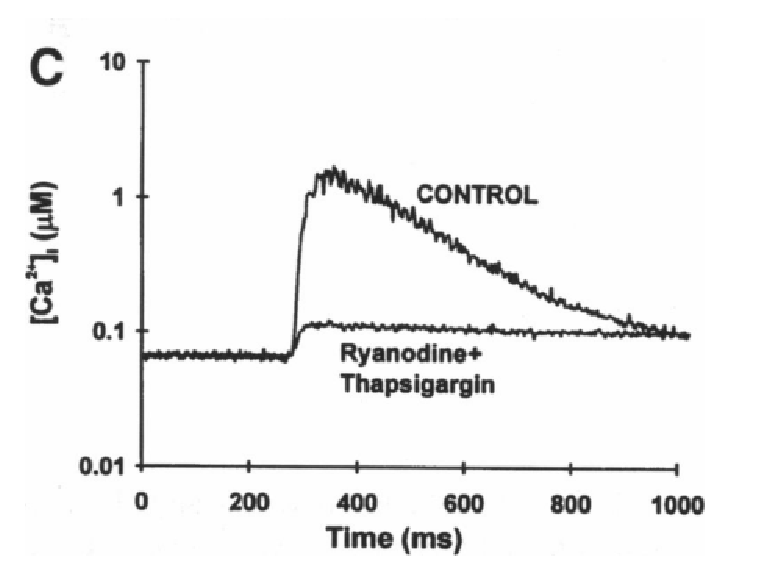
\includegraphics[height=4cm,
    angle=0]{./images/calcium_transient.eps}}
\caption{Plotting $[\Ca]_i$ in logarithmic scale in the presence of SR $\Ca$
inhibitors (1$\muM$ ryanodine to block SR $\Ca$ release and 1$\muM$ thapsigargin
to block $\Ca$ uptake through SERCA) \citep{cannell1994snu}. The $[\Ca]_i$
transient decrease from 1.57$\pm$0.1$\muM$ to 34$\pm$10.7 nM with the presence
of SR inhibitors}
\label{fig:calcium_transient}
\end{figure}

Regardless of many advances in modelling studies, two basic properties of
cardiac calcium dynamics is high gain and gradedness calcium release has not
been adequately resolved.
Early AP models belong to the so-called ``common-pool''
family~\citep{stern1992tec} (Chap.~\ref{chap:ap_ventricular_myocyte}), i.e. Ca
influx across sarcolemma and Ca release from SR are directed into a single
compartment which in turns control the SR release.
The single compartment can be the bulk myoplasm or the single ``common-pool''
models~\citep{jafri1998cad}, Fig.~\ref{fig:common_pool}.  In such models, as
soon as the Ca in the cytosol (or subspace) elevates enough to cause CICR, a
fully saturated release occurs so that the response is in a ``all-or-none''
behavior (i.e. high gain), rather than graded or ad-hoc formula need to be used.


\begin{figure}[hbt]
  \centerline{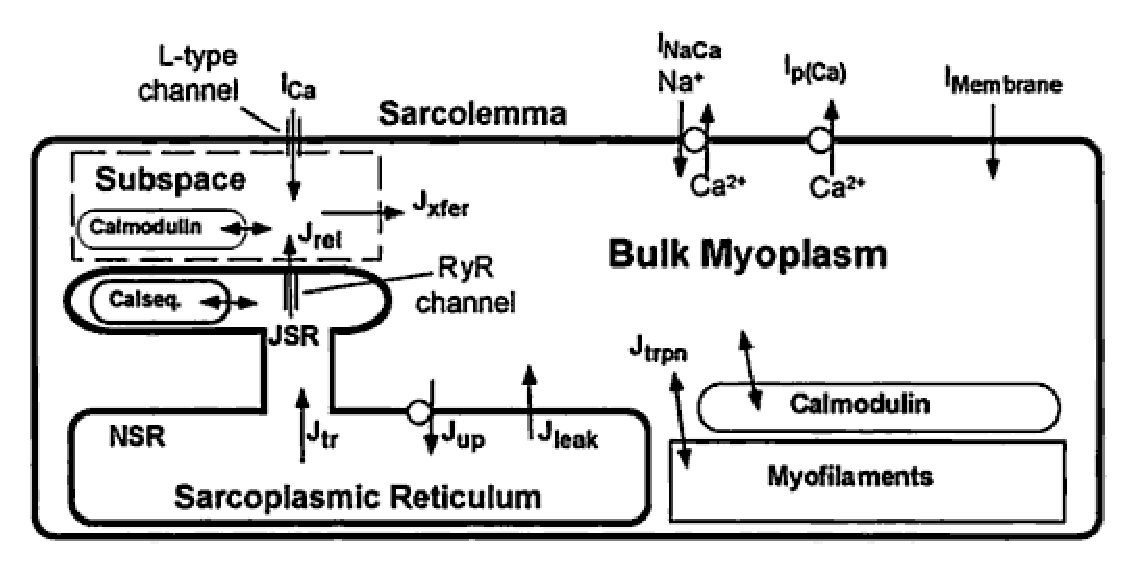
\includegraphics[height=5cm,
    angle=0]{./images/common_pool.eps}}
  \caption{Structure of a common pool model~\citep{jafri1998cad}}
  \label{fig:common_pool}
\end{figure}

\begin{framed}
  {\bf mechanistic vs. phenomenological (common-pool) models}:

  A mechanistic model should take into account the underlying
  biological process, while the phenomenological model basically can
  replicate the experimental results, without model the process in a
  realistic manner.

  Most common-pool models all show an all-or-none response. Some still
  can produce graded property by model the calcium release as a
  phenomenological function ({\it heuristic function}) of LCC influx
  and/or membrane potential, e.g. LR-2 model\citep{luo1994dmc_a} and
  its
  derivatives~\citep{fox2002,bondarenko2004cma,tenTusscher2004,hund2004,
    mahajan2008}.
  However, the approach may lack the predictive power of an approach
  that more closely represents the underlying mechanism.

  Later one, many evidences shown that $\Ca$ release is smoothly
  graded as a function of $\Ca$ trigger provided by the slow inward
  $I_{si}$~\citep{cannell1987,beuckelmann1988}.  This paradox is
  explained by the introduction local control
  theory~\citep{stern1992tec}.
\end{framed}

Common-pool models are useful, i.e. they can reproduce AP under normal and
pathological condition, \textcolor{blue}{it cannot describe the fundamental
property of graded
  junctional SR (JSR) $\Ca$ release?}~\citep{winslow2005mmc}.
To resolve this, stochastic implementation of the CRU need to be taken into
account with a large enough number of CRUs which requires much higher
computational demand (Chap.~\ref{chap:ap_ventricular_myocyte_localcontrol}).
~\citep{greenstein2002} developed the first comprehensive model based on the
theory of local control. It includes a small population of CRUs in which local
interaction of individual LCC and nearby RyRs are simulated stochastically. It
shown that LCC inactivation depend more strongly on local $\Ca$ than $V_m$.
However, this number of CRUs is far below the estimated number of CRUs per cell,
i.e. 20,000 CRUs.

Some efforts to reduce the computational demands by deriving a
simplified local control version of CICR~\citep{hinch2004slc}, and has
been applied to whole-cell model~\citep{tanskanen2006,
  greenstein2006}.  These models can reproduce all the core features
of previous models, yet with low computational demands, making a
candidate for large-scale tissue simulation. 

A full discussion of temporospatial model will be covered in
Chap.\ref{chap:3d-whole-cell}.




\section{What to test in a model}
\label{sec:what-test-model}

\subsection{$\Ca$ sparks}
\label{sec:calcium-sparks}

Spark rate, duration, magnitude




\subsection{Wenckebach periodicities}
\label{sec:wenck-peri}

Under normal condition, cells respond to stimulus under 1:1 ratio, i.e. one
stimulus one contraction of the cell. Under pathological conditions, e.g.
stimulus strength is too week, stimulus frequency is too fast, etc., the ratio
can be 2:1 (e.g. 2 stimulus cause a single contraction), complete block (no
contraction at all), or alternans (one stimulus cause long contraction, the
next one cause weak contraction)\ldots or Wenckebach rhythm. Wenckebach
periodicities in response to periodic stimulation.

Wenckebach rhythm was first found in AV node, which is characterized by a longer
APD and beat-t-beat increase in latency, causing a shorter APD in the next one
and culminating a skipped beat, after which the cycle repeats. Later one,
Wenckebach rhythm have  also been virtually found on other parts of the heart,
including ventricular myocytes \citep{anderson1972}. 

Under a complex interplay between delayed rectifier, inward rectifier, and fast
$\Na$ currents, it leads to a beat-to-beat increase in latency, producing a
beat-to-beat decrease in recovery time, eventually leading to a skipped beat. In
single rabbit ventricular cells, a dropped beat is followed by a longer APD. The
transient outward current $I_\to$ was accounted for this beat-to-beat increase
in APD during Wenckebach rhythm \citep{yehia1997}, Fig.\ref{fig:Wenckebach}.


\begin{figure}[hbt]
  \centerline{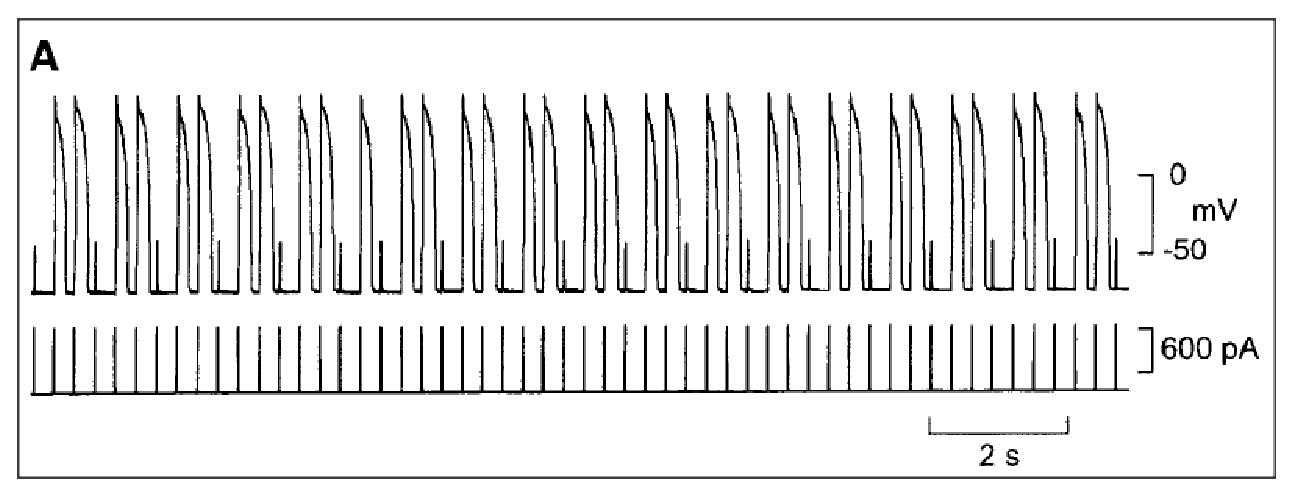
\includegraphics[height=4cm,
    angle=0]{./images/Wenckebach_3.2.eps}}
\caption{A 3:2 Wenckebach cycles interrupted by a single 2:1 cycle (at the 6th
cycle)}
\label{fig:Wenckebach}
\end{figure}

As we can see, there is not only a beat-to-beat increment in APD, but also the
beat-to-beat increase in latency. As $I_\to$ is known to activate in the early
phase of repolarization, this current has some role to this pathological
condition. The whole-cell transient outward current is modeled as
\begin{equation}	
I_\to = \overline{g}_\to.q.r.(V_m-E_\rev)
\end{equation}
$I_\to$ (pA), $\overline{g}_\to$ (nS) is the maximal conductance, the gating
variables: q (activation), and r (inactivation). They chose $E_\rev=-66$ (mV),
$\overline{g}_\to=5.6$ (nS) to give peak $I_\to$ the same as that found in
experiment. 


\subsection{$\Ca$ overload}
\label{sec:calcium-overload}

The experimental data with $[\Ca]_o$ increase from 1mM to 10mM, it increases the
frequency of spontaneous $\Ca$ spark to 4-fold, spark amplitude increase
4.1-fold, spatial size increases 1.7-fold \citep{cheng1996csc}. 

The transient inward current ($i_\ti$) is known to develop under Ca2+ overload
in cardiac cells (see review, Eisner \& Lederer, 1985). It has been attributed
to
\begin{enumerate}
  \item NCX current: 1$\Ca$ in : 3$\Na$ out

As $I_\ti$ disappears on replacing $\Na$ with $\Li$ (Arlock \& Katzung (1985)
and Brown, Noble, Noble \& Taupignon (1986)), it has been suggested that a
considerable part of $I_\ti$ is carried by NCX (Sect.\ref{sec:NCX_family}).
  
  \item $\Ca$-activated non-specific cation conductance (Kass, Lederer, Tsien \&
Weingart, 1978).
\end{enumerate}

Under $\Ca$ overload, this inward current causes the cell experiences periodic
spontaneous $\Ca$ sparks, and this release propagates as a ``calcium wave'', travelling
at a velocity in the range
$80-120\mu$m/s~\citep{stern1992tec}. Macroscopic waves has been
observed to propagates for milimeters at velocities up to 15mm/s. At the site
of wave initiation, $\Ca$ sparks were observed 65\% of the time
\citep{cheng1996csc}. 

To study the wave propagation over a wide range of SR calcium loads,
we can do subthreshold field stimulation, local application of
caffeine, or localized photo-release of caged calcium. 


\section{Pacing protocol}
\label{sec:pacing_protocol}

The AP clamp method is theoretically defined as $V_m=V_\rest$ (at rest) and
$V_m=V_\stim$ (during stimulation time).  However, numerically, the abrupt
change in $V_m$ from resting to stimulated value may cause unexpected numerical
issue. As a result, some developed options are:
\begin{enumerate}
  \item Use a ramping time, i.e. a short period of time for $V_m$ to increase
  and drop (linearly), i.e. 
  \begin{equation}
  V_m = \left\{ \begin{array}{cc}
  	V_\rest  & t < t_{\stim, start} \text{ and }	 t > t_{\stim, end} \\
  	V_\rest + (V_\stim-V_\rest) * (t-t_{\stim,start}) & \text{ if } t_{\stim,
  	start} < t < t_{\stim, start} + t_{ramp} \\
  	V_\stim - (V_\stim-V_\rest) * (t-t_{\stim,start}) & \text{ if } t_{\stim,
  	end} - t_{ramp} < t < t_{\stim, end}  
  \end{array}\right.
  \end{equation}
  \item Use ascending/descending function
  
  \item Use \citep{chudin1999icd} approach
  \begin{equation}
  V_m = \left\{ \begin{array}{cc}
  V_\rest & \text{ if }	mT + xT < t < (m+1)T \\
  V_\rest + (V_\stim - V_\rest) \times \sqrt{1 - \left( \frac{t-mT}{xT}
  \right)^2} & \text{ if }	mT \le t \le mT + xT
  \end{array} \right.
  \end{equation}
  
  with T is the period (pacing cycle length), $x=\APD/T$ with $m$ is the $m$-th
  beat. $x$ was fitted to experimental data using 
  \begin{equation}
  x(T) = \frac{a}{a+T}
  \end{equation}
\end{enumerate}

Many phenomena associated with EC-coupling depends on the stimulus interval.
This is known as {\bf interval-force relations} which describes the change in
force generation under high frequency of stimulation. \citep{jafri1998cad}
performed this test on the model (from 0.5Hz (after a long-enough time to
reach the steady state) to 1.5Hz and then going back to 0.5Hz after a certain
time period) and showed (1) a slightly smaller in AP peak, (2) a small increase
in the peak of $[\Ca]_i$ transient, (3) less RyR opening (due to refractory
causing a large fraction of RyR in the adapted states), which leading to (4)
higher SR calcium load, Fig.\ref{fig:Jafri1998_Fig8}.
Using 4Hz, the peak $[\Ca]_i$ transient is 0.92$\muM$, while at 1Hz, the peak is
0.84$\muM$ \citep{jafri1998cad}. Correspondingly, the diastolic $[\Ca]_i$ is
also higher, i.e. 0.19$\muM$ vs. 0.10$\muM$.

\begin{figure}[hbt]
  \centerline{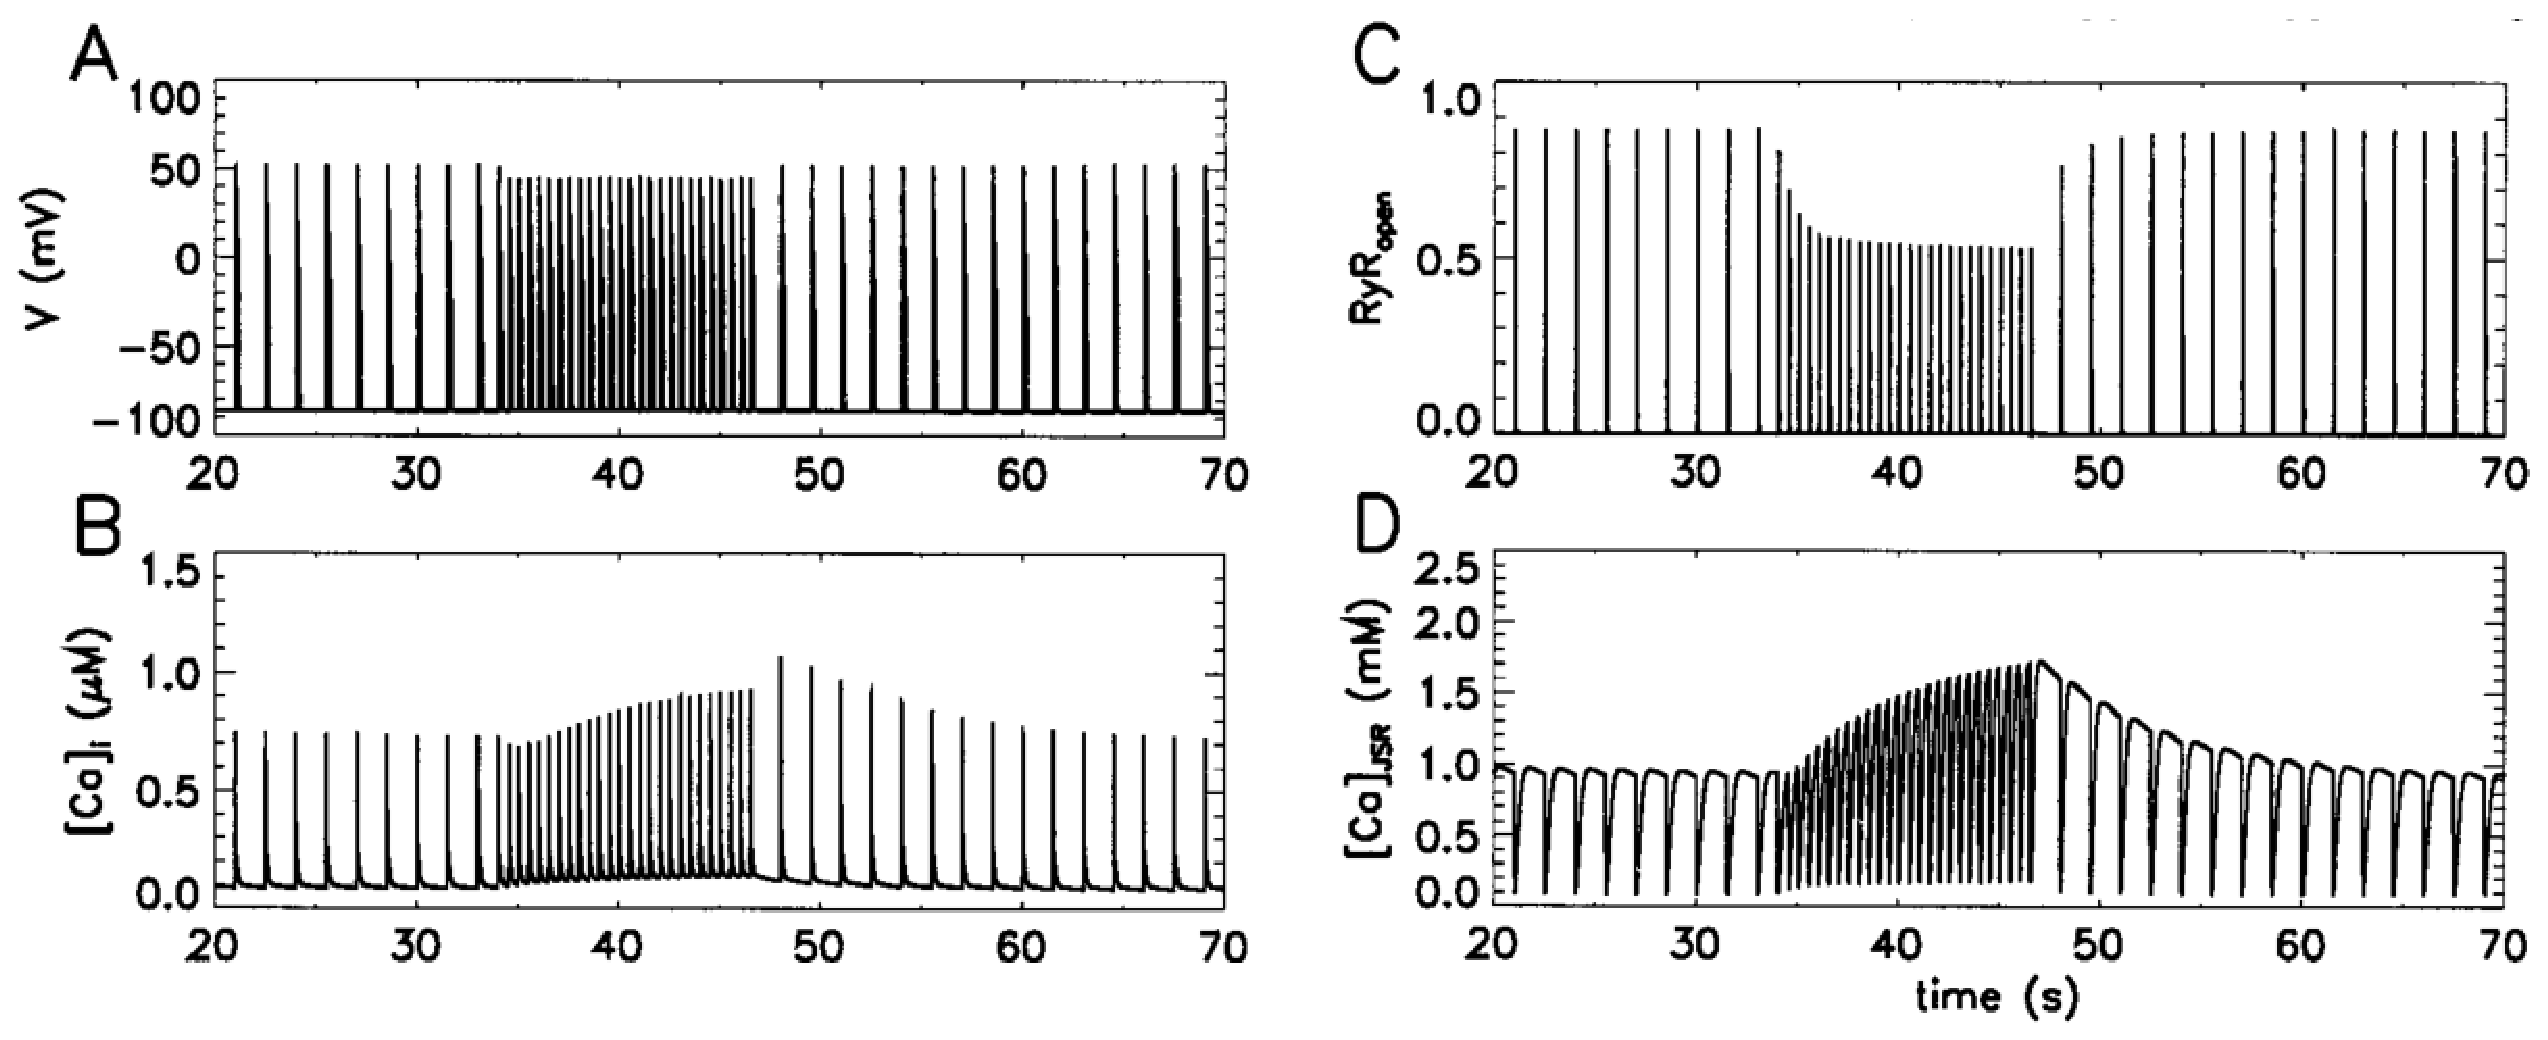
\includegraphics[height=5cm]{./images/Jafri1998_Fig8.eps}}
  \caption{Force-Interval relation}
  \label{fig:Jafri1998_Fig8}
\end{figure}



\section{Models for Human Ventricular Myocytes}

There have been so many models developed. However, the most importance of all
is models for human ventricular myocytes. In this section, we walk through a
number of models of this category.

The first human ventricular myocyte model is Priebe-Beuckelmann (1998)
(Sect.\ref{sec:priebe-beukelmann_1998}), and its simplification Bernus et. al. 
\citep{bernus2002}. The models were based on Luo-Rudy-2 for ventricular myocytes
(Sect.\ref{sec:luo-rudy-phase-2}) with parameters from human data.
\citep{tenTusscher2004} then updated the model with parameters of the membrane
currents are based on the more recent whole-cell data measured in isolated human
ventricular myocytes (Sect.\ref{sec:tenTusscher2004_human}). 

\citep{iyer2004} then extended the model so that $[\Ca]_i$ is more stability
over a range of pacing frequencies (Sect.\ref{sec:Iyer-Winslow2004}). 

